\documentclass[12pt]{article}
\usepackage[hmargin={.7in},vmargin={.7in}]{geometry}   
\geometry{letterpaper}       
%\geometry{landscape}          
%\usepackage[parfill]{parskip}
\usepackage{color,graphicx}
%\usepackage{covington}
%\usepackage{xyling}
\usepackage{setspace}
\usepackage{amsmath}
\usepackage{amssymb}
%\usepackage{graphicx,color}
%\usepackage{theorem}
%\usepackage{tabularx}
%\usepackage{subfig}
%\usepackage{vowel}
%\usepackage{mathrsfs}
\usepackage{varioref}
\usepackage{textcomp}
%\usepackage{avm}
\usepackage{textcomp}
\usepackage{mflogo}
\usepackage{wasysym}
%\usepackage{pstricks, pst-plot, pst-node, pst-tree, colortab}
%\usepackage{qtree}
 %\usepackage{tree-dvips}
 \usepackage{linguex}
%\usepackage{gb4e}
 \usepackage{multirow}
 %\usepackage[stable]{footmisc}
 \usepackage{pifont}
%\usepackage{todonotes}
%\usepackage{natbib}
\usepackage[normalem]{ulem}
\usepackage{wrapfig}

 %\setlength{\parskip}{.55ex plus 0.1ex}


\usepackage{fancyhdr} % This should be set AFTER setting up the page geometry
\pagestyle{plain} % options: empty , plain , fancy
\lhead{}\chead{}\rhead{}
\renewcommand{\headrulewidth}{.3pt}
\lfoot{}\cfoot{\thepage}\rfoot{}
%\renewcommand{\footrulewidth}{.3pt}
\newcommand{\txtp}{\textipa}
\renewcommand{\rm}{\textrm}
\newcommand{\sem}[1]{\mbox{$[\![$#1$]\!]$}}
\newcommand{\lam}{$\lambda$}
\newcommand{\lan}{$\langle$}
\newcommand{\ran}{$\rangle$}
\newcommand{\type}[1]{\ensuremath{\left \langle #1 \right \rangle }}
\newcommand{\defeq}{$\mathrel{\mathop:}=$ }
\renewcommand{\and}{$\wedge$ }


%\renewcommand{\Extopsep}{2pt}


\newcommand{\bex}{\begin{examples}}
\newcommand{\eex}{\end{examples}}

%bullet points
\newcommand{\bit}{\begin{itemize}}
\newcommand{\eit}{\end{itemize}}

%numbering, non sequential
\newcommand{\ben}{\begin{enumerate}}
\newcommand{\een}{\end{enumerate}}

\renewcommand{\abstractname}{The goal:}


%numbering, what you would use in a paper when you don't want the numbering to stop every time you end an example. 
%\newcommand{\bex}{\begin{enumerate}\setcounter{enumi}{\thesaveenumi}\item{}\begin{enumerate}}
%\newcommand{\eex}{\end{enumerate}\setcounter{saveenumi}{\theenumi}\end{enumerate}}

%%these are the brackets used for writing up semantic meanings 
%\newcommand{\lbr}{\textrm{\textlbrackdbl}}
%\newcommand{\rbr}{\textrm{\textrbrackdbl}}
%\renewcommand{\rm}{\textrm}

%this describes the numbering system (roman vs arabic numerals and so forth)
\renewcommand\theenumi {\alph{enumi}}
\renewcommand\theenumii {\alph{enumii}}
\renewcommand\labelenumi {\theenumi. }
\renewcommand\labelenumii {\theenumii.}
\labelformat{enumi}{(\theenumi)}
\labelformat{enumii}{(\theenumi\theenumii)}
\newcounter{saveenumi}

%\renewcommand{\labelitemi}{\textbf{---}}
%\renewcommand{\labelitemii}{\textbf{$\cdot$}}

%\linespread{1.5}

%\qtreecenterfalse

%\linespread{1}
%DIF PREAMBLE EXTENSION ADDED BY LATEXDIFF
%DIF UNDERLINE PREAMBLE %DIF PREAMBLE
\RequirePackage[normalem]{ulem} %DIF PREAMBLE
\RequirePackage{color}\definecolor{RED}{rgb}{1,0,0}\definecolor{BLUE}{rgb}{0,0,1} %DIF PREAMBLE
\providecommand{\DIFadd}[1]{{\protect\color{blue}\uwave{#1}}} %DIF PREAMBLE
\providecommand{\DIFdel}[1]{{\protect\color{red}\sout{#1}}}                      %DIF PREAMBLE
%DIF SAFE PREAMBLE %DIF PREAMBLE
\providecommand{\DIFaddbegin}{} %DIF PREAMBLE
\providecommand{\DIFaddend}{} %DIF PREAMBLE
\providecommand{\DIFdelbegin}{} %DIF PREAMBLE
\providecommand{\DIFdelend}{} %DIF PREAMBLE
%DIF FLOATSAFE PREAMBLE %DIF PREAMBLE
\providecommand{\DIFaddFL}[1]{\DIFadd{#1}} %DIF PREAMBLE
\providecommand{\DIFdelFL}[1]{\DIFdel{#1}} %DIF PREAMBLE
\providecommand{\DIFaddbeginFL}{} %DIF PREAMBLE
\providecommand{\DIFaddendFL}{} %DIF PREAMBLE
\providecommand{\DIFdelbeginFL}{} %DIF PREAMBLE
\providecommand{\DIFdelendFL}{} %DIF PREAMBLE
%DIF END PREAMBLE EXTENSION ADDED BY LATEXDIFF

\begin{document}

\begin{center}\textbf{Property subjectivity predicts adjective ordering preferences}
\end{center}

	\vspace{-15pt}

\DIFaddbegin \DIFadd{Cross-linguistically stable preferences for adjective ordering have been widely documented, yet the factors that determine these preferences are still poorly understood. }\DIFaddend Our approach to the investigation of adjective ordering preferences synthesizes strategies from the \DIFdelbegin \DIFdel{psychological approach}\DIFdelend \DIFaddbegin \DIFadd{\emph{psychological approach}}\DIFaddend , probing the principles that underlie these preferences \cite{sweet1898,ziff1960,martin1969determinants,martin1969competence,martin1970,kemmereretal2009}, and from the \DIFdelbegin \DIFdel{grammatical approach}\DIFdelend \DIFaddbegin \DIFadd{\emph{grammatical approach}}\DIFaddend , using descriptive semantic classes of adjective to structure and inform our hypotheses \cite{dixon1982,sproatshih1991,cinque1994,scott2002}. 
\DIFdelbegin \DIFdel{We first conducted a corpus study to measure, for }\DIFdelend \DIFaddbegin 

\DIFadd{\textbf{Exp.~1 (corpus study).} For }\DIFaddend 26 adjectives from seven different classes (size, quality, age, texture, shape, color, material; see Table 1 for the full list of adjectives\DIFdelbegin \DIFdel{tested), what their mean distance from the modified noun is in }\DIFdelend \DIFaddbegin \DIFadd{), we extracted all cases of }\DIFaddend phrases with either two or three adjectives (e.g., ``a good green color'' or ``some big new red cloaks'') \DIFdelbegin \DIFdel{. We extracted all such cases }\DIFdelend from the Switchboard \DIFdelbegin \DIFdel{corpus, as well as from both the written and spoken portions of }\DIFdelend \DIFaddbegin \DIFadd{and }\DIFaddend the British National Corpus (for a total of 39,199 cases). \DIFdelbegin \DIFdel{Mean }\DIFdelend \DIFaddbegin \DIFadd{For each adjective, we  computed its mean }\DIFaddend distance from the \DIFdelbegin \DIFdel{noun for each adjective class is }\DIFdelend \DIFaddbegin \DIFadd{modified noun. Means by adjective class are }\DIFaddend shown in Fig.~1 (corpus). \DIFdelbegin \DIFdel{Conducting pairwise }\DIFdelend \DIFaddbegin \DIFadd{Pairwise }\DIFaddend Bonferroni-corrected comparisons between classes on the \DIFdelbegin \DIFdel{average }\DIFdelend \DIFaddbegin \DIFadd{mean }\DIFaddend distance-from-noun scores \DIFdelbegin \DIFdel{calculated in Fig.~1 }\DIFdelend yields the following ordering preferences, which closely track the previous reports in the literature \cite{sproatshih1991,dixon1982}:
\DIFdelbegin %DIFDELCMD < \vspace{-13pt}
%DIFDELCMD < $$ %%%
\begin{displaymath}%DIFAUXCMD
\DIFdel{size \geq quality > age > texture > shape > color > material }%DIFDELCMD < \label{inferred-order-preferences}$$
%DIFDELCMD < %%%
\end{displaymath}%DIFAUXCMD
\DIFdelend %DIF > \vspace{-13pt}
\DIFaddbegin \DIFadd{\emph{size} $\geq$ \emph{quality} $>$  \emph{age} $>$  \emph{texture} $>$  \emph{shape} $>$  \emph{color} $>$  \emph{material} %DIF > \label{inferred-order-preferences}$$
}\DIFaddend 

\DIFdelbegin %DIFDELCMD < \vspace{-13pt}
%DIFDELCMD < %%%
\DIFdelend %DIF > \vspace{-13pt}

\DIFdelbegin \DIFdel{We closely replicated these }\DIFdelend \DIFaddbegin \DIFadd{\textbf{Exp.~2 (n=50)} closely replicated the }\DIFaddend inferred ordering preferences \DIFdelbegin \DIFdel{in a behavioral experiment, where we }\DIFdelend \DIFaddbegin \DIFadd{behaviorally. We }\DIFaddend elicited naturalness judgments on adjective-adjective-noun object descriptions, permuting the relative order of the adjectives. We used the same adjectives from the corpus experiment, paired at random with a set of ten nouns describing either food or furniture \DIFdelbegin \DIFdel{; }\DIFdelend \DIFaddbegin \DIFadd{(see Table 1 for }\DIFaddend the full list of words\DIFdelbegin \DIFdel{appears in Table 1.
Participants (n=50)}\DIFdelend \DIFaddbegin \DIFadd{).
Participants }\DIFaddend indicated which ordering of an adjective-adjective-noun object description sounded more ``natural,'' using a sliding scale with endpoints labeled with the competing object descriptions (e.g., ``the big red apple'' vs.\ ``the red big apple''). On the basis of these naturalness ratings, we computed for each adjective-adjective pairing its preferred, canonical order\DIFaddbegin \DIFadd{, by XXX}\DIFaddend . We then determined how often an adjective from a given semantic class occurred first in a preferred adjective-adjective-noun configuration; Fig.~1 (preference) plots these \DIFdelbegin \DIFdel{average distance }\DIFdelend \DIFaddbegin \DIFadd{mean distance XXX wait why distance? }\DIFaddend scores, where a value of 1 signals that a class's adjectives always occur first in preferred adjective-adjective-noun orderings. 

Having established the robustness of ordering preferences both in production (\DIFdelbegin \DIFdel{measured in our corpus experiment}\DIFdelend \DIFaddbegin \DIFadd{Exp.~1}\DIFaddend ) and in comprehension (\DIFdelbegin \DIFdel{measured in our naturalness rating experiment}\DIFdelend \DIFaddbegin \DIFadd{Exp.~2}\DIFaddend ), we then shifted focus to the source of these preferences. While researchers \DIFdelbegin \DIFdel{may disagree about its details, the }\DIFdelend \DIFaddbegin \DIFadd{disagree about the details, }\DIFaddend psychological explorations of ordering preferences \DIFdelbegin \DIFdel{converge }\DIFdelend \DIFaddbegin \DIFadd{have converged }\DIFaddend on the idea that aspects of  adjectives' meaning (\DIFdelbegin \DIFdel{i.e.}\DIFdelend \DIFaddbegin \DIFadd{e.g.}\DIFaddend , specificity, context-sensitivity, reliance on comparison\DIFdelbegin \DIFdel{, etc.}\DIFdelend ) determine their relative order \DIFdelbegin \DIFdel{.  On the basis of the preferred orderings we observed both in the corpus and in our behavioral experiment, we }\DIFdelend \DIFaddbegin \DIFadd{XXX refs?. %DIF >  On the basis of the preferred orderings we observed both in the corpus and in our behavioral experiment, 
We }\DIFaddend distilled the proposals that precede us into a single feature\DIFdelbegin \DIFdel{, }\DIFdelend \DIFaddbegin \DIFadd{: }\DIFaddend the subjectivity of the property named\DIFdelbegin \DIFdel{, as the single best predictor of ordering preferences. That is, in }\DIFdelend \DIFaddbegin \DIFadd{. In }\DIFaddend each of the observed preferred orderings, \DIFdelbegin \DIFdel{our intuitions, which we tested experimentally, suggested }\DIFdelend \DIFaddbegin \DIFadd{intuition suggests }\DIFaddend that less subjective adjectives appear closer to the modified noun. 

\DIFdelbegin \DIFdel{To measure }\DIFdelend \DIFaddbegin \DIFadd{\textbf{Exp.~3 (n=45)} tested this subjectivity hypothesis  by estimating }\DIFaddend the subjectivity of adjectives \DIFdelbegin \DIFdel{and the broader }\DIFdelend \DIFaddbegin \DIFadd{(and the }\DIFaddend classes to which they belong\DIFdelbegin \DIFdel{, we ran a second behavioral experiment. Participants (n=45) }\DIFdelend \DIFaddbegin \DIFadd{) using a faultless disagreement measure. Participants }\DIFaddend evaluated the potential for faultless disagreement between two differing descriptions of an object. For example, an experimental trial would have Mary assert ``that apple is old,'' then have Bob counter with ``that apple is not old.'' 
To the extent that both Mary and Bob can be right in their descriptions of the apple, ``old'' admits that degree of faultless disagreement. 
Thus, the extent to which two people can disagree about a description without one necessarily being wrong determines the subjectivity of that description. 
We validated \DIFdelbegin \DIFdel{our }\DIFdelend \DIFaddbegin \DIFadd{the }\DIFaddend faultless disagreement measure in a separate paradigm \DIFdelbegin \DIFdel{, which explicitly asked about the potential }\DIFdelend \DIFaddbegin \DIFadd{(n=XXX), in which participants rated the }\DIFaddend ``subjectivity'' of object descriptions \DIFaddbegin \DIFadd{directly}\DIFaddend ; the results of these two methods were highly correlated ($r^{2} = 0.89$), suggesting that \DIFdelbegin \DIFdel{the measures they invoked converge in their estimation of adjective }\DIFdelend \DIFaddbegin \DIFadd{faultless disagreement is a good proxy for }\DIFaddend subjectivity.

Fig.~1 (subjectivity) plots \DIFdelbegin \DIFdel{average }\DIFdelend \DIFaddbegin \DIFadd{mean }\DIFaddend faultless disagreement ratings for adjectives and their respective classes. Based \DIFaddbegin \DIFadd{on }\DIFaddend pairwise comparisons of these aggregate scores, we inferred the following adjective class subjectivity \DIFdelbegin \DIFdel{raking, which tracks the inferred order preference from the other experiments: 	}\DIFdelend \DIFaddbegin \DIFadd{ranking: 	\emph{quality} $\geq$ \emph{size} $>$ \emph{texture} $\geq$ \emph{age} $>$ \emph{color}
	$\geq shape \geq material$
}\DIFaddend \begin{wrapfigure}[47]{r}{.47\linewidth}
	%\vspace{-30pt}
	Table 1: The adjectives and their classes tested in all experiments, and the nouns and their classes tested in the behavioral experiments. \\
	{\footnotesize \begin{tabular}{llll}
		\textbf{adjective}	&	\textbf{class}	&	\textbf{adjective}	&	\textbf{class}	\\ \hline
		old	&	age	&	good	&	quality	\\
		new	&	age	&	bad	&	quality	\\
		rotten	&	age	&	round	&	shape	\\
		fresh	&	age	&	square	&	shape	\\
		red	&	color	&	big	&	size	\\
		yellow	&	color	&	small	&	size	\\
		green	&	color	&	huge	&	size	\\
		blue	&	color	&	tiny	&	size	\\
		purple	&	color	&	short	&	size	\\
		brown	&	color	&	long	&	size	\\
		wooden	&	material	&	smooth	&	texture	\\
		plastic	&	material	&	hard	&	texture	\\
		metal	&	material	&	soft	&	texture	\\
		\textbf{noun}	&	\textbf{class}	&	\textbf{noun}	&	\textbf{class}	\\ \hline
		apple	&	food	&	chair	&	furniture	\\
		banana	&	food	&	couch	&	furniture	\\
		carrot	&	food	&	fan	&	furniture	\\
		cheese	&	food	&	TV	&	furniture	\\
		tomato	&	food	&	desk	&	furniture	
	\end{tabular}}
	\vspace{-15pt}
	\begin{center}
		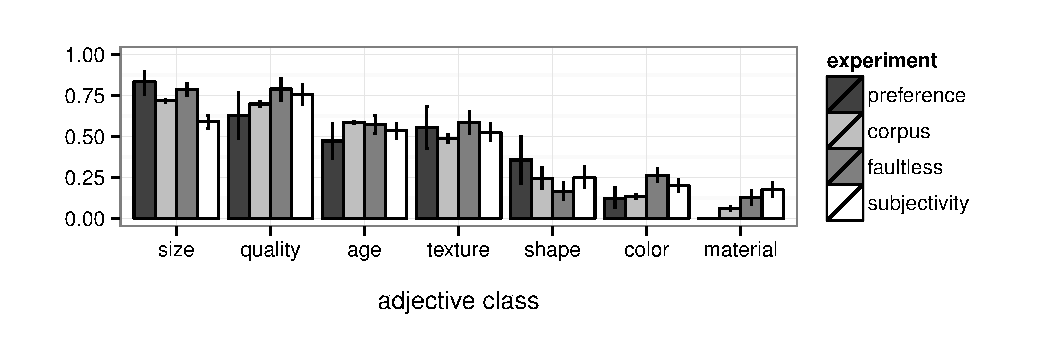
\includegraphics[width=.95\linewidth]{plots/expt_results.eps}
	\end{center}
	\vspace{-15pt}
	Fig.~1: \DIFdelbegin \DIFdel{Average }\DIFdelend \DIFaddbegin \DIFadd{Mean }\DIFaddend distance from noun (corpus), \DIFdelbegin \DIFdel{average }\DIFdelend \DIFaddbegin \DIFadd{mean }\DIFaddend preferred distance from noun  (preference), and \DIFdelbegin \DIFdel{average }\DIFdelend \DIFaddbegin \DIFadd{mean }\DIFaddend faultless disagreement scores (subjectivity) for adjectives by class.
	\vspace{-12pt}
	\begin{center}
		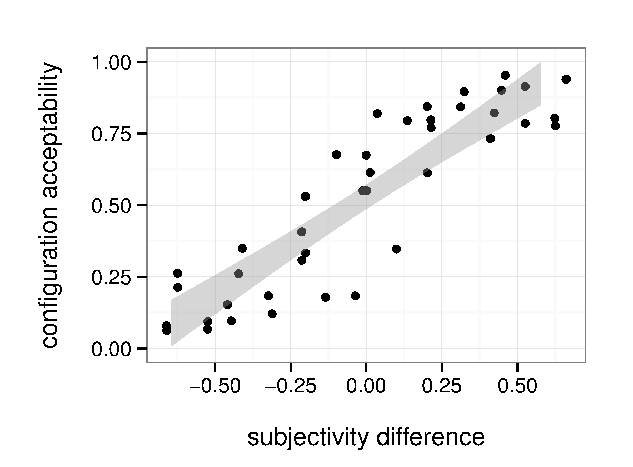
\includegraphics[width=.85\linewidth]{plots/comparison2.eps}
	\end{center}
	\vspace{-10pt}
	Fig.~2: Class-level order preferences plotted against faultless disagreement difference scores.
\end{wrapfigure}
\DIFdelbegin %DIFDELCMD < \vspace{0pt}
%DIFDELCMD < \vspace{-13pt}
%DIFDELCMD < \begin{center}
%DIFDELCMD < 	\vspace{-14pt}
%DIFDELCMD < 	%%%
\DIFdel{$quality \geq size > texture \geq age > color$}%DIFDELCMD < \\
%DIFDELCMD < 	%%%
\DIFdel{$\geq shape \geq material$
}%DIFDELCMD < \end{center}
%DIFDELCMD < \vspace{-11pt}
%DIFDELCMD < %%%
\DIFdelend %DIF > \vspace{0pt}
%DIF > \vspace{-13pt}
%DIF > \begin{center}
%DIF > 	\vspace{-14pt}
%DIF > 	$quality \geq size > texture \geq age > color$\\
%DIF > 	$\geq shape \geq material$
%DIF > \end{center}
%DIF > \vspace{-11pt}

\noindent
\DIFaddbegin \DIFadd{This ranking closely tracks the inferred order preferences from Exps.~1 and 2.
}\DIFaddend To evaluate the \DIFdelbegin \DIFdel{predictive }\DIFdelend power of subjectivity in \DIFdelbegin \DIFdel{determining }\DIFdelend \DIFaddbegin \DIFadd{predicting }\DIFaddend adjective order, we compared \DIFdelbegin \DIFdel{acceptability ratings from the preference experiment with }\DIFdelend \DIFaddbegin \DIFadd{naturalness ratings (Exp.~2) to }\DIFaddend faultless disagreement scores \DIFdelbegin \DIFdel{. We  calculated }\DIFdelend \DIFaddbegin \DIFadd{(Exp.~3). We  computed }\DIFaddend a subjectivity difference score for each class configuration (i.e., an ordered pairing of two adjective classes, class1-class2) by subtracting the \DIFdelbegin \DIFdel{average }\DIFdelend \DIFaddbegin \DIFadd{mean }\DIFaddend faultless disagreement score for \textsc{class1} from the \DIFdelbegin \DIFdel{average }\DIFdelend \DIFaddbegin \DIFadd{mean }\DIFaddend faultless disagreement score for \textsc{class2}. Higher difference scores indicate that the adjective class closer to the noun is less subjective than the class farther away. Fig.~2 plots \DIFdelbegin \DIFdel{acceptability }\DIFdelend \DIFaddbegin \DIFadd{naturalness }\DIFaddend ratings  against these faultless disagreement difference scores; the two measures are highly correlated ($r^2$ = 0.81), strongly supporting \DIFdelbegin \DIFdel{our }\DIFdelend \DIFaddbegin \DIFadd{the }\DIFaddend hypothesis that less subjective adjectives occur more closely to the noun.

Adjective ordering preferences have received considerable attention throughout the history of generative grammar and cognitive psychology, owing to its remarkable stability within and across languages. Something so robust, the reasoning goes, must evidence a deep principle of the cognitive architecture that shapes language. Yet while descriptions of the phenomenon abound, an explanation continues to prove elusive. Our findings serve to narrow the space of possible explanations: rather than representing these preferences as a fully specified ranking according to semantic classes or syntactic projections, our results demonstrate that ordering preferences more likely emerge from a desire to place more informative, less subjective content closer to the substantive head of a nominal construction (i.e., closer to the modified noun).

\noindent
\footnotesize
	\textbf{References:} 
	[1]  Sweet (1898), {\em A New English Grammar};
	[2]  Ziff (1960), {\em Semantic Analysis};
	[3]  Martin (1969), {\em Semantic Determinants of Preferred Adjective Order}, J.~of Verbal Learning and Verbal Behavior, 8, 697--704;
	[4]  Martin (1969), {\em Some Competence-Process Relationships in Noun Phrases with Prenominal and Postnominal Adjectives}, J.~of V.~Learning and V.~Behavior, 8, 471--480;
	[5]  Martin (1970), {\em Adjective Order and Juncture}, J.~of V.~Learning and V.~Behavior, 9, 379--383;
	[6] Kemmerer, Tranel \& Zdansczyk (2009). {\em Knowledge of the semantic constraints on adjective order can be selectively impaired}, J.~of Neurolinguistics, 22, 91--108;
	[7]  Dixon (1982), {\em Where have all the adjectives gone?, and other essays in semantics and syntax};
	[8]  Sproat \& Shih (1991). {\em The cross-linguistic distribution of adjective ordering restrictions}, Interdisciplinary approaches to language: Essays in honor of S.-Y.~Kuroda (1991), 565--593;
	[9]  Cinque (1994), {\em On the evidence for patial N-movement in the Romance DP}, Paths towards Universal Grammar. Studies in honor of Richard S.~Kayne, 85--110;
	[10]  Scott (2002), {\em Stacked adjectival modification and the structure of nominal phrases}, The Cartography of Syntactic Structures, 91--120.

	
\newpage

\begin{thebibliography}{10}

	\bibitem{sweet1898}
	H.~Sweet, {\em A New English Grammar} (1898).

	\bibitem{ziff1960}
	P.~Ziff, {\em Semantic Analysis} (1960).

	\bibitem{martin1969determinants}
	J.~E.~Martin, {\em Semantic Determinants of Preferred Adjective Order}, Journal of Verbal Learning and Verbal Behavior, 8 (1969), pp.~697--704. 

	\bibitem{martin1969competence}
	J.~E.~Martin, {\em Some Competence-Process Relationships in Noun Phrases with Prenominal and Postnominal Adjectives}, Journal of Verbal Learning and Verbal Behavior, 8 (1969), pp.~471--480. 

	\bibitem{martin1970}
	J.~E.~Martin, {\em Adjective Order and Juncture}, Journal of Verbal Learning and Verbal Behavior, 9 (1970), pp.~379--383. 

	\bibitem{kemmereretal2009}
	kemmerer

	\bibitem{dixon1982}	
	R.~M.W.~Dixon, {\em Where have all the adjectives gone?, and other essays in semantics and syntax} (1982).

	\bibitem{sproatshih1991}
	R.~Sproat and C.~Shih, 1991. {\em The cross-linguistic distribution of adjective ordering restrictions}, Interdisciplinary approaches to language: Essays in honor of S.-Y.~Kuroda (1991), pp.~565--593.

	\bibitem{cinque1994}
	G.~Cinque, {\em On the evidence for patial N-movement in the Romance DP}, Paths towards Universal Grammar. Studies in honor of Richard S.~Kayne (1994), pp.~85--110.

	\bibitem{scott2002}
	G.-J.~Scott, {\em Stacked adjectival modification and the structure of nominal phrases}, The Cartography of Syntactic Structures (2002), pp.~91--120.
\end{thebibliography}


%\bibliographystyle{chicago}
%\bibliography{greg.bib}




\end{document}






\noindent
\begin{minipage}[t]{.48\linewidth}
	\vspace{0pt}
	\begin{center}
		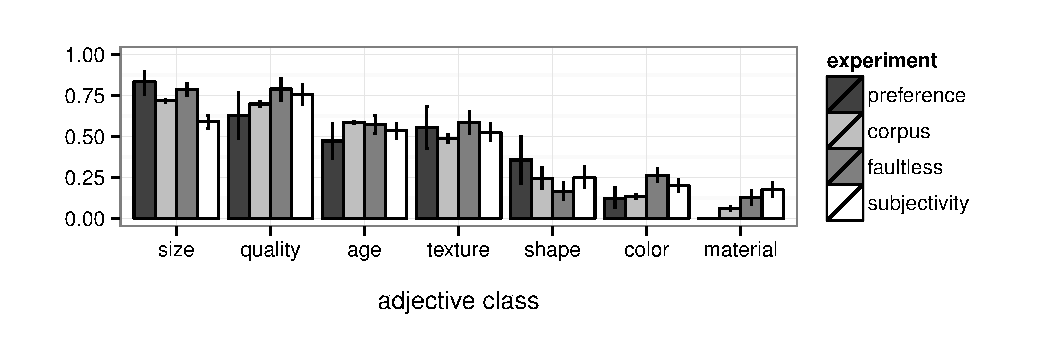
\includegraphics[width=\linewidth]{plots/expt_results.eps}
	\end{center}
	\vspace{-15pt}
	Fig.~1 (corpus results): Mean distance from noun by adjective class for cases with at least two modifying adjectives.
	Fig.~2 (Expt.~1 results): Mean preferred distance from noun for each adjective class.
	Fig.~3 (Expt.~2 results): Mean faultless disagreement scores for adjectives by class.
\end{minipage} \hfill
\begin{minipage}[t]{.46\linewidth}
	\vspace{0pt}	
	\begin{center}
		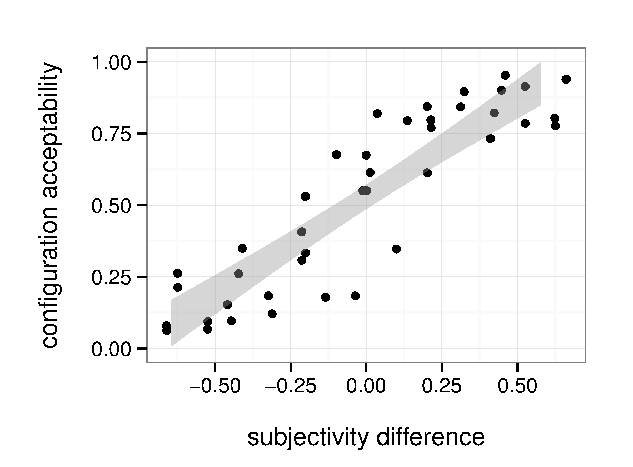
\includegraphics[width=\linewidth]{plots/comparison2.eps}
	\end{center}
	Fig.~4: Class-level order preferences plotted against difference in faultless disagreement between A1 and A2 (values greater than 0 indicate that the more subjective adjective class occurs farther from the noun).
\end{minipage}